s%%%%%%%%%%%%%%%%%%%%%%%%%%%%%%%%
\section{The Photon Detection System}
\label{sec:detectors-fd-ref-pd}

The scope of the photon detector (PD) system for the DUNE far detector
reference design includes design, procurement, fabrication,
testing, delivery and installation:
\begin{itemize}
\item light collection system including wavelength shifter and light guide
\item silicon photo-multipliers (SiPMs)
\item readout electronics
\item calibration system
\item related infrastructure (frames, mounting boards, etc...)
\end{itemize}

Liquid argon is an excellent scintillating medium and the photon
detection system will exploit this property in the far detector.  With
an average energy needed to produce a photon of 19.5~eV (at zero
field) a typical particle depositing 1~MeV in liquid argon will
generate 40,000~photons with wavelength of 128~nm. At higher fields
this will be reduced but at 500~V/cm the yield is still
$\sim$20,000~photons per MeV. Roughly 1/4 of the photons are promptly
emitted with a lifetime of about 6~ns while the rest have a lifetime
of 1100--1600~ns. LAr is highly transparent to the 128~VUV photons
with a Rayleigh scattering length of (66~$\pm$~3)~cm~\cite{Rayleigh}
and absorption length of $>$200~cm\footnote{This attenuation length
  requires a LN2 content of less than 20~ppm}. The relatively large light yield
makes the scintillation process an excellent candidate for
determination of $t_{0}$ for non-beam related events. Detection of the
scintillation light may also be helpful in background rejection and
triggering on non-beam events.

The photon detection system reference design described in this section
meets the required performance for light collection for the DUNE far
detector. The photon system will provide the t$_0$ timing of events
relative to TPC timing with a resolution better than 1~$\mu$s
(providing position resolution along drift direction of a few mm)
allowing determination of proton decay location with reasonably high
efficiency.  Alternate designs may allow even higher proton decay
efficiency and allow PD measurement of even lower energy phenomena
such as supernovae neutrinos.

Figure~\ref{fig:PD_overview} shows the layout for the photon detector
system, which will be described in the following sections.
\begin{cdrfigure}[PD Overview]{PD_overview}{Overview of the PD
    system showing a cartoon schematic (a) of a single PD module
    in the LAr and the channel ganging scheme used to reduce the
    number of readout channels. Panel (b) shows how each PD module
    will be inserted into an APA frame. There will be 10 PDs instered
    into an APA frame.}
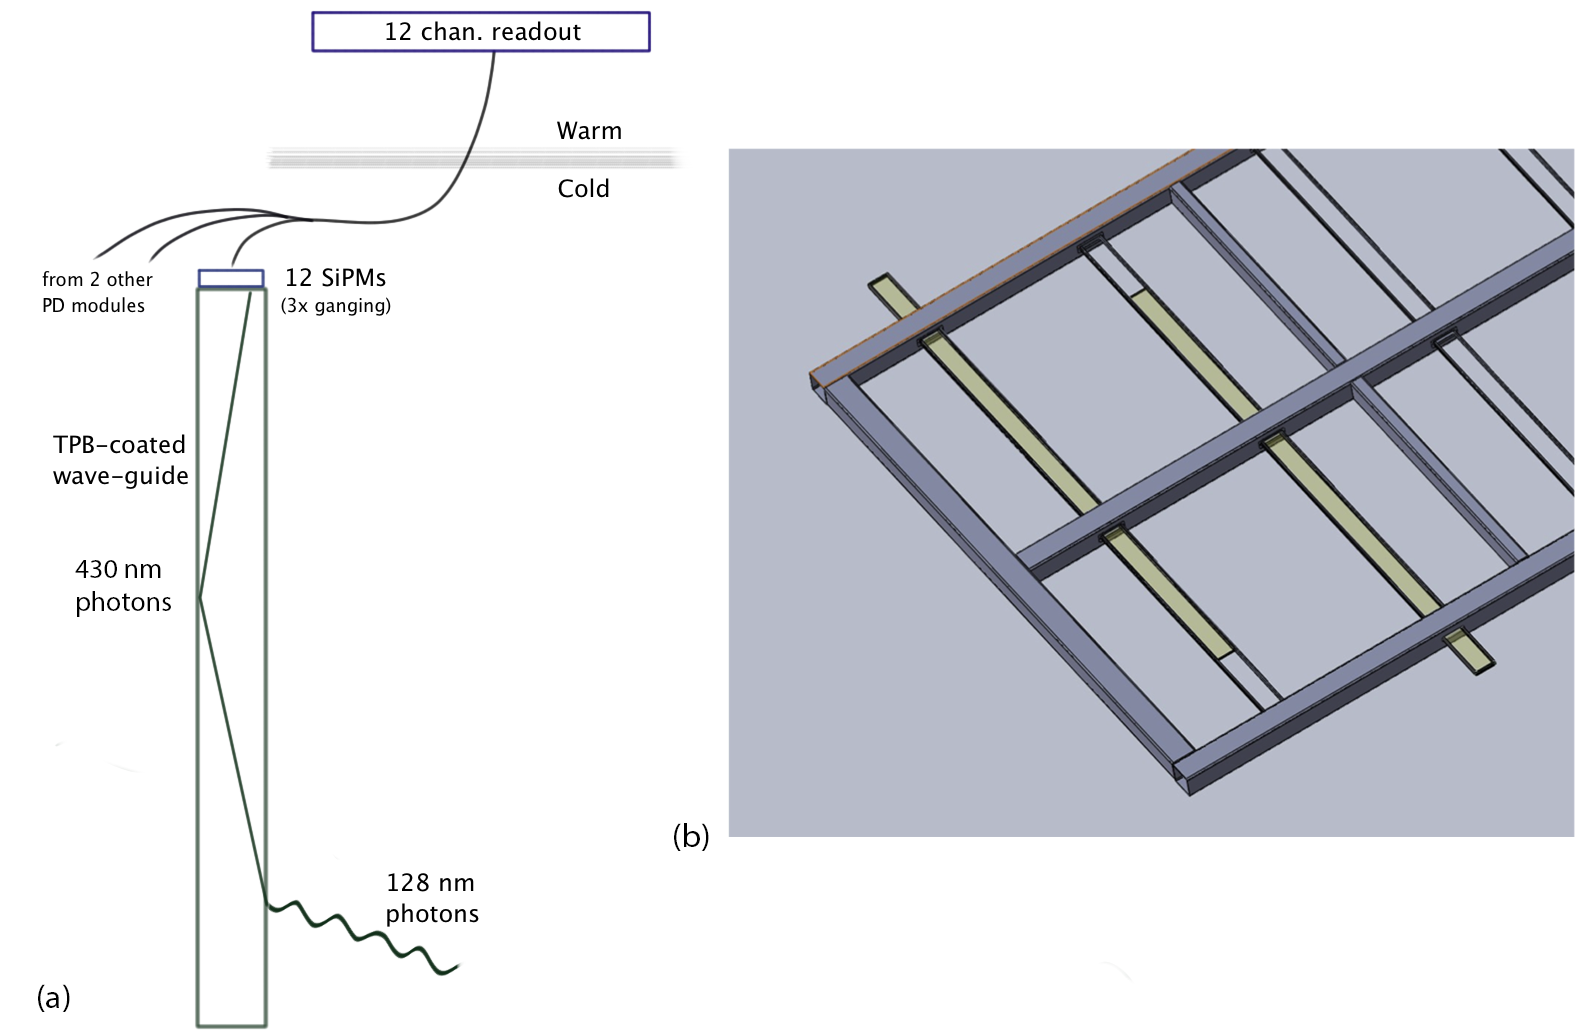
\includegraphics[width=1.0\linewidth]{pd_schem.png}
\end{cdrfigure}

\subsection{Reference Design}
\label{sec:detectors-fd-ref-pd-refsystem}   % Refer to SSP description in this section from DAQ section

The PD system is mounted on the APA frames.  To enable this, the
reference design for mounting the PDs into the APA frames calls for
ten PD modules\footnote{A PD module is the combination of light-guide
and SiPMs.} (Figure~\ref{fig:PD_overview}~(a)), approximately 2.2-m
long, 83-mm wide, and 6-mm thick, equally spaced along the full length
of the APA frame (Figure~\ref{fig:PD_overview}~(b)).

The 128-nm scintillation photons from liquid argon interact with the
wavelength shifter on the light guide, or bar, surface and the light
peaked around 430-nm is re-emitted in the bar. The light guide
transports the wavelength-shifted light to 12 silicon
photo-multipliers (SiPMs) mounted at one end of the bar.

The wavelength shifter converts the scintillation photons striking the
bar surface and directs them into the bar bulk with an efficiency of
$\sim$50\%.  A fraction of the waveshifted optical photons are
internally reflected to the bar's end where they are detected by SiPMs
with quantum efficiency well matched to the wavelength-shifted
photons. The light guides are made with a coating of TPB
(1,1,4,4-tetraphenyl-1,3-butadiene). A testing program is currently
underway to determine the absolute performance of the light guides in
liquid argon.

The SiPMs used in the reference design are SensL C-Series 6~mm$^2$
(MicroFB-60035-SMT) devices. These SiPMs have detection efficiency of
41\%\footnote{The detector efficiency combines QE and effective areal
  coverage accounting for dead space between pixels.} While the
C-Series SensL SiPMs are not rated for operation below
$-$40$^{\circ}$~C their performance has been excellent for this
application. At LAr temperature (89~K) the dark rate is of order 10~Hz
(0.5 p.e. threshold) while after-pulsing has not been an
issue. Extensive testing is underway to ensure that the SiPMs can
reliably survive the stresses associated with thermal cycling in LAr
and long-term operation at LAr temperature.

The SiPMs are read out using shielded twisted-pair cable, one per SiPM,
but the expected final design will have three SiPMs ganged together and
each readout cable will contain four individual channel cables to keep
the cost and cable packing density down. During the R\&D phase of the
project each SiPM was read out in order to ensure maximum information
was gathered during tests.  

The front-end electronics reside outside of the cryostat in
instrumentation racks. A custom module for receiving SiPM signals has
been designed and built. The module also performs signal processing in
the front-end as preprocessing for trigger and DAQ.  The module is
called the SiPM Signal Processor (SSP) and consists of 12 readout
channels packaged in a self-contained 1U module.  Each channel
contains a fully-differential voltage amplifier and a 14-bit, 150-MSPS
analog-to-digital converter (ADC) that digitizes the waveforms
received from the SiPMs. There is no shaping of the signal, since the
SiPM response is slow enough relative to the speed of the digitization
to obtain several digitized samples of the leading edge of the pulse
for the determination of signal timing. Digitized data is processed by
a Xilinx Artix-7 Field-Programmable Gate Array (FPGA).  The use of the
FPGA processing allows for a significant amount of customization of
the SSP operation. 

Once the DUNE collaboration arrives at a refined set of physics
requirements for the photon detection system a set of criteria for a
calibration system will be determined. In the absence of such criteria
two calibration systems have are being explored, and will be tested in
the 35-t phase-II test. The first system, developed by ANL, utilizes 5
fiber-fed diffusers mounted on the TPC CPA which uniformly illuminate
the photon detectors. An alternate design is employed on the IU
prototypes and uses LED-driven fibers mounted alongside the
waveguides. 

\subsection{Alternative Designs} 

Three alternative designs are currently being considered for the PD
system.

The first alternative is based on a TPB-coated acrylic panel with an
embedded S-shaped wavelength-shifting fiber. The Louisiana State
University (LSU) group has developed prototypes based on this design
in an attempt to allow an increase in detector size and hence increase
geometric acceptance of the PD system and hence reduce overall system
cost.

In this design, a single acrylic panel PD module has the same
dimensions as the reference design and consists of a TPB-coated
acrylic panel with an embedded multi-lobed ``S-shaped'' wavelength
shifting (Y11) fiber. The fiber is read out by two SiPMs (one on the
top edge, and the other on the bottom edge of the plate), which are
coupled to either end of the fiber and serve to transport the light
over long distances with minimal attenuation. The double-ended fiber
readout has the added benefit of providing some position dependence to
the light generation along the panel by comparing relative signal
sizes and arrival times in the two SiPMs. The WLS fiber converts the
430-nm light from the TPB to light with a peak intensity of
480--500~nm, which is well-matched to the peak photon-detection
efficiency of typical SiPMs.

A second alternative prototype, under investigation by the Colorado
State University (CSU) group, utilizes blue-green (Y11)
wavelength-fibers. The prototype has a thin TPB-coated acrylic
radiator located in front of a close-packed array of WLS fibers. The
motivation for this design was to address an issue with the reference
design, in which the application of TPB to acrylic, or other base
materials, has been found to cause a significant decrease in
attenuation length (down to about 30~cm) of the light guide. The
prototype is two-sided and has two identical fiber arrays and
radiators mounted back-to-back with a tyvek refelctor between. This
design allows for a reduction in the number of SiPMs required per PD
module. Three SiPMs per side are needed per PD module (again the same
dimensions in length and width as the reference design) for a total of
six SiPMs per PD module.

The Indiana University (IU) group has advanced CSU design and arrived
at the third alternative design by replacing the Y11 fiber with a
reference-design-dimensioned cast bar doped (by Eljen Technology) with
the same wavelength shifter as the Y11 fiber. The TPB-coated acrylic
radiator has also been replaced with a thin-fused silica plate coated
with TPB. This prototype has demonstrated an attenuation length
greater than 2.5~m and early indications seem to indicate that it
could meet the SN neutrino energy requirement. It is the ``brightest''
prototpye tested so far.

\subsection{Technology Selection}

The alternative designs have all demonstrated the ability to detect
LAr scintillation light, and development work is continuing. A testing
program is underway comparing the various alternatives against the
reference design.  The Tallbo large dewar at Fermilab and the
cryogenic detector development facility at CSU are being used to
compare the performance of full-scale and near-full-scale prototypes
in LAr utilizing alpha sources and cosmic muons. Data from the 35-t
prototype will also provide input into the technology decision. In
Fall 2015 a decision will be made regarding which design to adopt and
optimize for the first 10-kt far detector module.
